\documentclass[MAS331_Note.tex]{subfiles}

\begin{document}
\chapter{Countability and Separation Axioms}
\section{The Countability Axioms}

\dfn{First Countability Axiom}{
    A topological space $X$ is said to have a \textit{countable basis at} $x$
    if there is a countable collection $\mcal B$ of neighborhoods of $x$ in $X$
    such that, for each neighborhood $U$ of $x$, there exists $B \in \mcal B$
    with $B \subseteq U$. A space that has a countable basis at each point is
    said to satisfy the \textit{first countability axiom}, or to be
    \textit{first-countable}.
}

\nt{
    This definition was already given in \Cref{def:1stCt}.
    Recall the lemmas \Cref{lem:seqLemma} and \Cref{lem:seqConvIffImgConv}.
}

\dfn{Second Countability Axiom}{
    If a topological space $X$ has a countable basis for its topology, then
    $X$ is said to satisfy the \textit{second countability axiom}, or to be
    \textit{second-countable}.
}

\exmp{}{
    $\RR[J]$ endowed with the product topology with a countable set $J$ is
    second-countable;
    \[
        \mcal S \triangleq \bigcup_{\alpha \in J} \big\{\, \pi_{\alpha}\inv
        \big((a, b)\big) \:\big|\: a, b \in \QQ \text{ and } a<b \big\}
    \]
    is a countable subbasis for $\RR[J]$, which induces a countable basis for
    $\RR[J]$.
}

\nt{
    If a topological space $X$ is second-countable with a countable basis
    $\mcal B= \{B_n\}_{n \in \ZZ_+}$ and a subspace $A \subseteq X$ with the
    discrete topology. Then, $A$ must be countable.

    Otherwise, for each $a \in A$, there exists $B_a \in \mcal B$ such that
    $B_a \cap A = \{a\}$. This induces an injection $A \hookrightarrow \mcal B$.
    Hence, $A$ is countable.
}

\exmp[RUnifNot2ndCt]{Uniform Topology and Countability Axioms}{
    In the uniform topology, $\RR[\omega]$ is first-countable by
    \Cref{exmp:metIs1stCt}. Let $\mcal B$ be a basis of $\RR[\omega]$. Let
    \[
        A \triangleq \big\{\,(x_i)_{i \in \ZZ_+} \in \RR[\omega] \:\big|\:
        \forall i \in \ZZ_+,\: x_i \in \{\,0, 1\,\}\,\big\}\text{.}
    \]
    Then, $A$ has the discrete topology but $A$ is uncountable. Therefore,
    $\RR[\omega]$ with the uniform topology is not second-countable.
}

\thm[subspCt]{}{
    Let $X$ be a topological space and $A$ be a subspace of $X$.
    \begin{itemize}[nolistsep]
        \ii If $X$ is first-countable, then $A$ is first-countable.
        \ii If $X$ is second-countable, then $A$ is second-countable.
    \end{itemize}
}
\pf{Proof}{
    \hfill
    \begin{itemize}[nolistsep]
        \ii Let $a \in A$. Let $\mcal B$ be a countable basis of $X$ at $a$.
            Then, $\{\,B \cap A \mid B \in \mcal B\,\}$ is a countable basis
            for the subspace $A$ at $a$. \checkmark
        \ii Let $\mcal B$ be a countable basis of $X$. Then, $\{\,B \cap A
            \mid B \in \mcal B\,\}$ is a countable basis for the subspace $A$.
            \checkmark
    \end{itemize}
}

\thm[prodCt]{}{
    Let $\{X_\alpha\}_{\alpha \in J}$ be a countable family of topological
    spaces.
    \begin{itemize}[nolistsep]
        \ii If each $X_i$ is first-countable, then $\prod_{\alpha \in J}
            X_\alpha$ in the product topology is first-countable.
        \ii If each $X_i$ is second-countable, then $\prod_{\alpha \in J}
            X_\alpha$ in the product topology is second-countable.
    \end{itemize}
}
\pf{Proof}{
    \hfill
    \begin{itemize}[nolistsep]
        \ii Let $(x_{\alpha})_{\alpha \in J} \in \prod_{\alpha \in J} X_\alpha$.
            Then, for each $\alpha \in J$, there exists a countable basis
            $\mcal B_\alpha$ of $X_\alpha$ at $x_\alpha$.
            Then, $\big\{\, \prod_{\alpha \in J} B_\alpha \:\big|\:
            \forall \alpha \in J,\: B_\alpha \in \mcal B_\alpha\,\big\}$ is a
            countable basis at $(x_\alpha)_{\alpha \in J}$.
        \ii For each $\alpha \in J$, there exists a countable basis $\mcal
            B_\alpha$ of $X_\alpha$. Then, $\big\{\,\prod_{\alpha \in J}
            B_\alpha \:\big|\: \forall \alpha \in J,\: B_\alpha \in \mcal
            B_\alpha\,\big\}$ is a countable basis of $\prod_{\alpha \in J}
            X_\alpha$.
    \end{itemize}
}

\dfn{Lindelöf Space}{
    A topological space $X$ is called a \textit{Lindelöf space} if, for every
    open covering of $X$, there is a countable subcovering.
}

\dfn{Dense Subset}{
    A subset $A$ of a topological space $X$ is said to be \textit{dense} in $X$
    if $\cl A = X$.
}

\dfn{Separable Space}{
    A topological space $X$ is said to be \textit{separable} if there is a
    countable dense subset of $X$.
}

\nt{
    Obvious facts:
    \begin{itemize}[nolistsep]
        \ii Every compact space is a Lindelöf space.
        \ii The box and product topologies on an finite product of separable
            spaces is separable.
            (\Cref{th:prodOfClosureIsClosureOfProd})
        \ii Every topology on a countable set is Lindelöf and separable.
   \end{itemize}
}

\thm[2ndCtThenLindAndSep]{}{
    Let $X$ be a second-countable space. Then,
    \begin{itemize}[nolistsep]
        \ii $X$ is a Lindelöf space.
        \ii $X$ is separable.
    \end{itemize}
}
\pf{Proof}{
    Let $\mcal B = \{B_n\}_{n \in \ZZ_+}$ be a countable basis for $X$.
    \begin{itemize}[nolistsep]
        \ii Let $\mcal A$ be an open covering of $X$. For each $n \in \ZZ_+$,
            there exists $A_n \in \mcal A$ such that $B_n \subseteq A_n$.
            Then, $\mcal A' \triangleq \{\,A_n \mid n \in \ZZ_+\,\}$ is a
            countable subcovering of $X$ as $\mcal B$ covers $X$. \checkmark
        \ii For each $n \in \ZZ_+$, choose $x_n \in B_n$. Let $D \triangleq
            \{\,x_n \mid n \in \ZZ_+\,\}$. Then, for all $x \in X$, every
            basis element that contains $x$ intersects $D$; $\cl D = X$
            by \Cref{th:inClosureIffNeighCapANonempty}. \checkmark
    \end{itemize}
}

\exmp[REllCt]{$\RR_\ell$ and Countability Axioms}{
    \begin{itemize}[nolistsep]
        \ii Given $x \in \RR_\ell$, $\{\,[x, x + 1/n) \mid n \in \ZZ_+\,\}$
            is a countable basis at $x$. $\RR_\ell$ is first-countable.
        \ii $\cl{\QQ} = \RR_\ell$. $\RR_\ell$ is separable.
        \ii Let $\mcal B$ be a basis for $\RR_\ell$. Choose, for each $x \in
            \RR_\ell$, an element $B_x \in \mcal B$ such that $x \in B_x
            \subseteq [x, x+1)$. If $x \neq y$, then $B_x \neq B_y$. Hence
            $x \mapsto B_x$ is an injection; $\mcal B$ is uncountable.
            Therefore, $\RR_\ell$ is not second-countable.
    \end{itemize}
    We now prove $\RR_\ell$ is Lindelöf. Thanks to \Cref{lem:topByBIsUnionsOfB},
    we only have to prove that, for any open covering $\mcal A$ of $\RR_\ell$
    by the basis elements, there is a countable subcovering.

    Let $\mcal A = \{\,[a_\alpha, b_\alpha) \mid \alpha \in J\,\}$ be an open
    covering of $\RR_\ell$. Let $C \triangleq \bigcup_{\alpha \in J} (a_\alpha,
    b_\alpha)$. We now claim that $\RR \setminus C$ is countable.
    Let $x \in \RR \setminus C$. Then $x = a_\beta$ for some $\beta \in J$.
    Choose $q_x \in \QQ$ such that $q_x \in (a_\beta, b_\beta)$.
    If $x, y \in \RR \setminus C$ and $x < y$, then $q_x < q_y$. Hence
    $x \mapsto q_x$ defines an injection $\RR \setminus C \hookrightarrow \QQ$.
    Therefore, $\RR \setminus C$ is countable.

    Now, let $\mcal A'$ be a countable subcollection of $\mcal A$ that covers
    $\RR \setminus C$. Now, note that $\{\,(a_\alpha, b_\alpha) \mid \alpha \in
    J\,\}$ is an open covering of $C$ as a subspace of $\RR$ (with the standard
    topology). Since $\RR$ is second-countable, there exists a finite
    subcollection $\{\,(a_{\alpha_1}, b_{\alpha_1}), \cdots, (a_{\alpha_n},
    b_{\alpha_n})\,\}$ covers $C$. Let $\mcal A'' \triangleq \{\,[a_{\alpha_1},
    b_{\alpha_1}), \cdots, [a_{\alpha_n}, b_{\alpha_n})\}$.
    Then, $\mcal A' \cup \mcal A''$ is a countble subcovering of $\RR_\ell$.
}

\exmp[sorgenfrey]{The Product of Two Lindelöf Spaces Need Not Be Lindelöf}{
    Although $\RR_\ell$ is Lindelöf, $\RR_\ell \times \RR_\ell$ is not.
    Consider the subspace $L \triangleq \{\,x \times (-x) \mid x \in
    \RR_\ell\}$. Then, $L$ has the discrete topology as $\big([x, x+1) \times
    [-x, -x+1)\big) \cap L = \{x \times (-x)\}$. Hence, $L$ is not Lindelöf;
    $\RR_\ell^2$ is not Lindelöf.
}

\exmp{A Subspace of a Lindelöf Space Need Not Be Lindelöf}{
    The ordered square $I_o^2$ is compact (\Cref{exmp:orderedSqIsCpt}) and thus
    is Lindelöf. However, the subspace $A = I \times (0, 1)$ is not Lindelöf
    as an open covering $\{\,\{x\} \times (0, 1) \mid x \in I\,\}$ does not
    allow a countable subcovering.
}

\nt{
    Here is the diagram that represents the relations between spaces.
    \begin{center}
    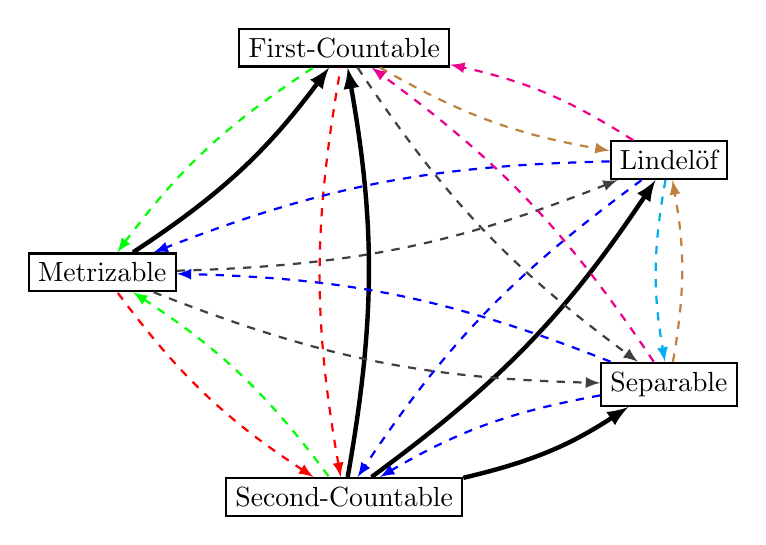
\begin{tikzpicture}[thick]
        \node[draw] (met) at (180:4) {Metrizable};
        \node[draw] (first) at (108:3) {First-Countable};
        \node[draw] (second) at (-108:3) {Second-Countable};
        \node[draw] (lind) at (24:3.5) {Lindelöf};
        \node[draw] (sep) at (-24:3.5) {Separable};

        \draw[->, >=latex, bend right=10, ultra thick] (met) edge (first);
        \draw[<-, >=latex, bend left=10, green] (met) edge[dashed] (first);
        \draw[->, >=latex, bend right=10, ultra thick] (second) edge (first);
        \draw[<-, >=latex, bend left=10, red] (second) edge[dashed] (first);
        \draw[<-, >=latex, bend left=10, green] (met) edge[dashed] (second);
        \draw[<-, >=latex, bend left=10, red] (second) edge[dashed] (met);
        \draw[->, >=latex, bend right=10, ultra thick] (second) edge (lind);
        \draw[->, >=latex, bend right=10, ultra thick] (second) edge (sep);
        \draw[->, >=latex, bend right=10, blue] (lind) edge[dashed] (met);
        \draw[->, >=latex, bend right=10, blue] (sep) edge[dashed] (met);
        \draw[->, >=latex, bend right=10, blue] (lind) edge[dashed] (second);
        \draw[->, >=latex, bend right=10, blue] (sep) edge[dashed] (second);
        \draw[->, >=latex, bend right=10, brown] (sep) edge[dashed] (lind);
        \draw[->, >=latex, bend right=10, brown] (first) edge[dashed] (lind);
        \draw[->, >=latex, bend right=10, darkgray] (met) edge[dashed] (lind);
        \draw[->, >=latex, bend right=10, darkgray] (met) edge[dashed] (sep);
        \draw[->, >=latex, bend right=10, darkgray] (first) edge[dashed] (sep);
        \draw[->, >=latex, bend right=10, magenta] (sep) edge[dashed] (first);
        \draw[->, >=latex, bend right=10, magenta] (lind) edge[dashed] (first);
        \draw[->, >=latex, bend right=10, cyan] (lind) edge[dashed] (sep);
    \end{tikzpicture}
    \end{center}

    Counterexamples:
    \begin{itemize}[nolistsep]
        \ii ({\color{green}$\dashrightarrow$}) $X = \{0, 1\}$ with $\mcal T =
            \{\varnothing, X, \{0\}\}$ is second-countable but not Hausdorff,
            thus not metrizable.
        \ii ({\color{red}$\dashrightarrow$})
            $\RR[\omega]$ with the uniform topology is metrizable but not
            second-countable. (\Cref{exmp:RUnifNot2ndCt})
        \ii ({\color{blue}$\dashrightarrow$})
            $\RR_\ell$ ($\RR$ with the lower limit topology) is
            first-countable, Lindelöf, and separable; but it is neither
            second-countable nor metrizable. (\Cref{exmp:REllCt})
        \ii ({\color{brown}$\dashrightarrow$})
            $\RR_\ell \times \RR_\ell$ is first countable and separable, but
            it is not Lindelöf. (\Cref{exmp:sorgenfrey})
        \ii ({\color{darkgray}$\dashrightarrow$})
            $\RR$ with the discrete topology is first-countable and metrizable;
            but it is not second-countable, separable, or Lindelöf.
        \ii ({\color{magenta}$\dashrightarrow$})
            $\RR$ with the finite complement topology is separable and
            Lindelöf; but it is neither first-countable nor metrizable.
        \ii ({\color{cyan}$\dashrightarrow$})
            $\RR$ with the countable complement topology is Lindelöf;
            but it is not first-countable, metrizable, or separable.
    \end{itemize}
}

\end{document}
